\chapter{Implementacja}
\label{cha:implementacja}

W działaniu programu można wyodrębnić 2 główne etapy, jest to dostarczenie danych zgonych formatem aplikacji a następnie ich wyświetlenie. Zapewniono obsługę zewnętrznych plików, zarówno zapisanych w standardzie KML jak i jego rozszeżenia stworzonego na potrzeby projektu. Interpretacja graficzna danych została zoptymalizowana na potrzeby pracy z dużymi zbiorami danych, tak aby wyświetlenie nawet dużej ilości informacji umożliwiało dalszą pracę.


\section{Struktura projektu}
\label{sec:structure}

Struktura klas w aplikacji została stworzona w oparciu o wzorzec projektowy MVC(en. Model–view–controller). Zakłada on podział na 3 główne warstwy, są nimi:

\begin{itemize}
\item
Controller - jego zadaniem jest przyjmowanie danych wejściowych i na ich podstawie odpowiednia reakcja, która może być aktualizają modelu lub warstwy prezentacyjenj.  W aplikacji funkcję tą spełniają servisy i kontrolery.
\item
View - warstwa prezentacyjna, zapewnia wizualiną prezentację infrmacji. Rolę tą w omwianym projekcie spełnia HTML i CSS.
\item
Model - przechowuje dane, stanowi bazę danych. Jego rola została przeniesiona na natywne rozwiązanie jakim jest Storage.
\end{itemize}

Założenia wzorca nie zostały w pełni spełnione, jego adaptacja została wykonana na potrzeby omawianego projektu. Stworzono podstawy do rozwoju i prostej adaptacji rozwiązania do potrzeb konkretnego klienta, w bardzo prosty sposób można zmienić między innymi sposób przechowywania danych aby spełnić wymagania klienta.


Zastosowano również paradygmat odwrócenego sterowania(en. Inversion of control,IoC) polegający na przeniesieniu poza obiekt metod służących do kontroli jego poszczególnych elementów. Główną zaletą tego podejścia jest uproszczona kongiguracja programu do potrzeb użytkownika. Przykładem zastosowania jest metoda korzystania z filtrów w aplikacji, które mogą być tworzone przez użytkownika. Ich potencjalnie duża ilość wczytywana jednocześnie podczas startu generowałaby zbędne obciążenie, obecnie są one pomijane podczas inicjacji i wczytywane pojedyńczo jedynie wtedy gdy ich obecność jest niezbędna.


Struktura klas obecnych w aplikacji została zaperzentowana na rysunku \ref{fig:classDiagram2}.

\begin{center}
\begin{figure}[H]
\centering
     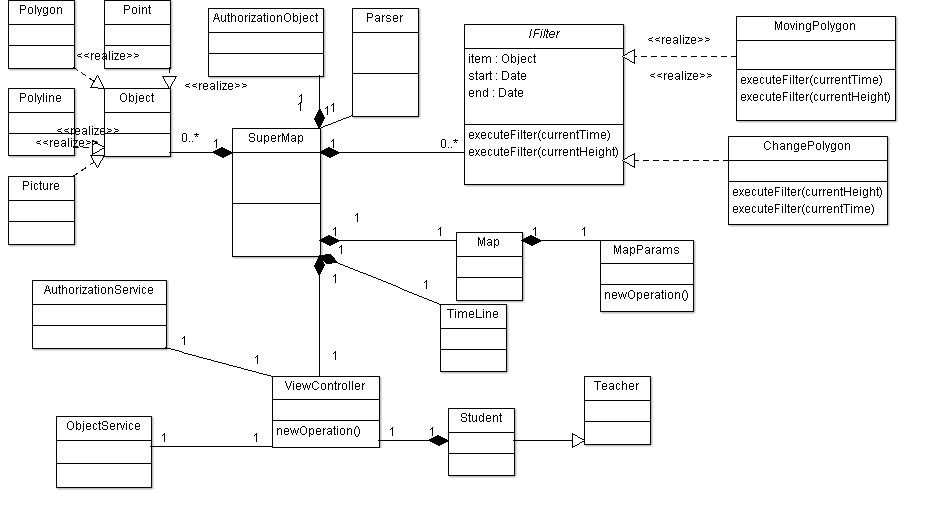
\includegraphics[angle=270,origin=c,width=130mm]{ge/smieci/ClassDiagram.png}
      \caption{Diagram klas.}
       \label{fig:classDiagram2}
\end{figure}
\end{center}

\section{Minimalna konfiguracja}
\label{sec:minimum}

Do rozpoczęcia korzystania z gotowej aplikacji należy zapewnić obecność konfiguracji niezbędnej do jej konfiguracji na docelowej stronie. Przykład minimalnej wersji która spełnia wymagane został pokazany w listinu \ref{lst:minconf}.

Z uwagi na naturę projektu, aplikacja wykorzystywana w przeglądarce, jak każdy dokument stworzony w HTML musi składać się z 3 głównych części:


-lini zawierającej informację o używanej wersji HTML, w poniższym przykładzie dotyczy ona HTML5

-deklaracji sekcji header, zawiera odwołania do zewnętrzych plików i delkaracje funcji, styli

-część właściwa strony która zawiera infromacje właściwe, widoczne dla użytkownika storny.

Linie 5-7 mają za zadanie wczytanie zewnętrzych plików zawierające delkaracje metod w JS. 8 wczytuje plik zawierający główną klasę frameworku, poniżej znajduje się wczytanie niezbędnych styli CSS dla działąnia osi czasu. 13-23 jest to opis metody która inicjuje działanie mapy, jest ona wykonywana po załadowaniu statycznych fragmentów strony.

\lstset{language=JavaScript}
\begin{lstlisting}[label={lst:minconf},caption={Minimalna konfiguracja.}]

<!DOCTYPE html>
<html>
  <head>
    <script type="text/javascript" src="https://maps.googleapis.com/maps/api/js?sensor=false&key={KEY_ID}">
    <script type="text/javascript" src="./js/specialMap/lib/jquery-1.6.2.min.js"></script>
    <script type="text/javascript" src="./js/specialMap/lib/mxn/mxn.js?(googlev3)"></script>
    <script type="text/javascript" src="./js/specialMap/lib/timeline-1.2.js"></script>
    <script type="text/javascript" src="./js/specialMap/src/timemap.js"></script>
    <script type="text/javascript" src="./js/specialMap/src/utils.js"></script>

    <link type="text/css" rel="stylesheet" href="./css/examples.css"/>

    <script>
    var sm;
    $(function() {
        tm = SpecialMap.init({
            mapDivId: "mapId",
            timeDivId: "timeId",
            dataType: "sessionStorage",
            bandIntervals: [
	            Timeline.DateTime.YEAR
	        ],
        });
    });
  </head>
  <body>
        <div id="specialMap">
            <div id="timeId"></div>
            <div id="mapId"></div>
        </div>
  </body>
</html>
\end{lstlisting}/


\section{Interfers do map}
\label{sec:mxn}

W procesie badań literaturowych podjęto decyzję aby jako głównego źródła map wykorzystać Google Maps \ref{subsec:Rodzaje map}.Postanowiono jednocześnie umożliwić użytkownikowi możliwość zmiany i wyboru innego dostarczyciela danych. Niestety nawet krótka analiza interfejsów dostarczaych do pracy nad różnymi typami map wskazuje na brak kompatybilności pomiędzy nimi, oznacza to brak możliwości stworzenia jednej implementacji działąjącej na różnych typach. Problem ten rozwiazano potrzez wykorzystanie Mapstraction, biblioteki której zadaniem jest płynne przechodzenie pomiędzy różnymi dostarczycielami i ich interfejsami.

Listening \ref{lst:mapstraction} pokazuję przykład wykorzystania biblioteki. Stworzenie instancji Mapstraction polega na wywołaniu konstruktora z podaniem id elementu który znajduje się na stronie i będzie używany jako nasza mapa a także typ mapy. Rezultatem jest obiekt kóry posiada wspólny interjeft dla różnych dostarzcycieli danych.

\lstset{language=JavaScript}
\begin{lstlisting}[label={lst:mapstraction},caption={Wykorzystanie Mapstraction.}]

var map = new Mapstraction(mapId, 'google');

var point = new mxn.LatLonPoint(0,0);
var marker = new mxn.Marker(point);
map.addMarker(marker);

\end{lstlisting}/



\section{Odczyt danych}
\label{sec:idata}

Tak jak zostało omówione w sekcji \ref{sec:dataformat} do przechowywania danych stworzono format rozszeżający istniejący obecnie KML.Takie podejście pozwala na swobodne tworzenie i edycję plików wejsciowych, brak ograniczeń. Jednocześnie zachowując minimalną strukturę obecnie istniejącego formatu pozwala na dostęp od dużej bazy istniejących informacji.

W celu odczytu i konwersji danych z pliku zapisu ich w pamięci sesyjnech przęglądarki omówionej w rozdziale \ref{subsec:storage5} stworzona została klasa FileParser. Posiada ona jednoargumentowy konstruktor przyjmujący ciąg znakowy będący zawartośćią pliku .

Ze względów bezpieczeństwa JavaScript nie zezwala na bezpośredni dostęp do plików lokalnych uzytkownika. Jest to pozytywne zachowanie zapewniające że żaden kod nie jest w stanie bezwiednie zmieniać zawartość dysku.

Wymusza to korzystanie z event-ów które będą aktywowane w momecie kiedy plik zostanie wybrany. W momencie zakończenia procesu odczytu zawartość pliku przekazywana jest do parsera który zapisuje dane w pamięci przeglądarki.

W przeciwieństwie do języków które posiadają klasyczną koncepcję klasy JavaScript posiada jedynie obiekt, z uwagi na ten fakt tworzenie metod i procedur następuje odmiennie. Istnieją 3 podstawowe sposby:

\begin{itemize}
\item
Wykorzystanie globalnej funkcji. Tworzony obiekt zawiera odowłanie do ciała metody, które jest globalne. Wadą takiego rozwiązania jest tworzenie wielu globalnym funkcji których nazwa może kolidować z nazwazmi w wykorzystywanych bibliotekach.
\item
Stworzenie funkcji wewnętrzej. Podobnie jak w poprzednim przypadku tworzona jest funkcja , tym razem jej ciało znajduje się w obiekcie. Minusem jest konieczność odtwarzania metody przy każdej sytuacji tworzenia obiektu. Operacja taka może być kosztowna i negatywnie wpływać na pracę aplikacji.
\item
Protototypowanie. Posiadając definicję obiektu możemy dodać do niego metodę. Sposób ten nie posiada wad opisanych powyżej, z tego powodu podejście zostało wykorzystane w stworzonej aplikacji. Przykład można zaobserwować w listeninu \ref{lst:svgImpl}.
\end{itemize}

\lstset{language=JavaScript}
\begin{lstlisting}[label={lst:utils},caption={Minimalna konfiguracja.}]

var exml;
function readFile(file,start,stop){
	var reader = new FileReader();
    reader.onloadend = function(evt) {
      if (evt.target.readyState == FileReader.DONE) {
		exml = new FileParser( evt.target.result);	
		exml.parse()
      }
    };
	
	var blob = file.slice(start, stop);
    reader.readAsBinaryString(blob);
}


\end{lstlisting}/


\lstset{language=JavaScript}
\begin{lstlisting}[label={lst:minconf},caption={Parser plików.}]

KmlParser.value = function(e) {
	a = GXml.value(e);
	a = a.replace(/^\s*/, "");
	a = a.replace(/\s*$/, "");
	return a;
}

KmlParser.prototype.createMarker = function(point,begin, end, name, desc, style, iconUrl) {
	var icon = {};
	var markeroptions = this.opts.markeroptions || {};
	var icontype = this.opts.icontype || "style";
	if (icontype == "style") {
		if (!!this.styles[style]) {
			icon = this.styles[style];
		}
	}
	if (!markeroptions.icon) {
		markeroptions.icon = icon;
	}
	var m = new google.maps.Marker(point, markeroptions);

	if (this.opts.elabelclass) {
		var l = new ELabel(point, name, this.opts.elabelclass,
				this.opts.elabeloffset, this.elabelopacity, true);
	}
	this.gmarkers.push(m);
	item = {};
	item.start = begin;
	item.end = begin;
	item.title = name;
	item.desc = desc;
	item.iconUrl = iconUrl;
	p = {};
	p.lat = point.lat();
	p.lon = point.lng();
	item.point = p
	return item;
}

KmlParser.prototype.createPolyline = function(points, color, width, opacity,
		name, desc) {
	var polylineoptions = this.opts.polylineoptions || {};
	var p = new GPolyline(points, color, width, opacity, polylineoptions);
	this.gpolylines.push(p);

KmlParser.prototype.createPolygon = function(points, id, pId, begin, end, color,
		width, opacity, fillcolor, fillopacity, name, desc) {

	pointsArray = []
	item = {};
	for ( var i = 0; i < points.length; i++) {
		point = points[i];
		p = {};
		p.lat = point.lat();
		p.lon = point.lng();
		if (p.lon == null || p.lat == null || isNaN(p.lat) || isNaN(p.lon)) {
			console.log("Null points");
		} else {
			pointsArray.push(p)
		}
	}
	item.start = begin;
	item.end = end;
	item.polygon = pointsArray;
	item.title = name;
	item.mId = id;
	item.pId = pId;
	item.color = color;
	item.width = width;
	item.opacity = opacity;
	item.fillcolor = fillcolor;
	item.name = name;
	item.desc = desc;

	return item;
}

KmlParser.prototype.processing = function(doc) {
	var that = this;
	var xmlDoc = GXml.parse(doc)
	
	var styles = xmlDoc.documentElement.getElementsByTagName("Style");
	for ( var i = 0; i < styles.length; i++) {
			//wczytanie styli
	}

	var placemarks = xmlDoc.documentElement.getElementsByTagName("Placemark");
	items = [];
	itemsMarkers = [];
	for ( var i = 0; i < placemarks.length; i++) {
		var id = placemarks[i].getAttribute('id');
		var timeSpan = placemarks[i].getElementsByTagName("TimeSpan")[0];
		var begin = KmlParser.value(timeSpan.getElementsByTagName('begin')[0])
		var end = KmlParser.value(timeSpan.getElementsByTagName('end')[0])
		var name = KmlParser.value(placemarks[i].getElementsByTagName("name")[0]);
		var desc = KmlParser.value(placemarks[i]
				.getElementsByTagName("description")[0]);
		if (desc == "") {
			var desc = KmlParser
					.value(placemarks[i].getElementsByTagName("text")[0]);
			desc = desc.replace(/\$\[name\]/, name);
			desc = desc.replace(/\$\[geDirections\]/, "");
		}
		if (desc.match(/^http:\/\//i)) {
			desc = '<a href="' + desc + '">' + desc + '</a>';
		}
		if (desc.match(/^https:\/\//i)) {
			desc = '<a href="' + desc + '">' + desc + '</a>';
		}
		var style = KmlParser.value(placemarks[i]
				.getElementsByTagName("styleUrl")[0]);
		var coords = GXml.value(placemarks[i]
				.getElementsByTagName("coordinates")[0]);

		var path = coords.split(" ");

		multiGeometry = getChildrenTag(placemarks[i], 'MultiGeometry')[0];
		if(multiGeometry){
			allPolygons = multiGeometry.getElementsByTagName("Polygon")
		}else{
			allPolygons = {};
		}
		
		onePoint = getChildrenTag(placemarks[i], 'Point')[0];
		if (!!that.styles[style]) {
					var width = that.styles[style].width;
					var color = that.styles[style].color;
					var opacity = that.styles[style].opacity;
					var fillopacity = that.styles[style].fillopacity;
					var fillcolor = that.styles[style].fillcolor;
					var iconUrl = that.styles[style].iconUrl;
				} else {
					var width = 5;
					var color = "#0000ff";
					var opacity = 0.45;
					var fillopacity = 0.25;
					var fillcolor = "#0055ff";
				}
		
		if(onePoint){
			coords = GXml.value(onePoint.getElementsByTagName("coordinates")[0]);
				var bits = coords.split(",");
				var point = new google.maps.LatLng(parseFloat(bits[1]),
						parseFloat(bits[0]));
				that.bounds.extend(point);
					itemsMarkers.push(that.createMarker(point ,begin,end, name, desc, style, iconUrl));
		}
		
		for ( var j = 0; j < allPolygons.length; j++) {
			polygon = allPolygons[j];
			coords = GXml.value(polygon.getElementsByTagName("coordinates")[0]);
			path = coords.split(" ");

			if (path.length > 1) {
				var points = [];
				var pId = polygon.getAttribute('id');
				for ( var p = 0; p < path.length; p++) {
					var bits = path[p].split(",");
					if (parseFloat(bits[1]) == null
							|| parseFloat(bits[0]) == null
							|| isNaN(parseFloat(bits[1]))
							|| isNaN(parseFloat(bits[0]))) {
					} else {
						var point = new google.maps.LatLng(parseFloat(bits[1]),
								parseFloat(bits[0]));
						points.push(point);
					}
				}
				this.pointsCount  = this.pointsCount + points.length;
				var linestring = placemarks[i]
						.getElementsByTagName("LineString");
				if (linestring.length) {
						that.createPolyline(points, color, width, opacity,
								name, desc);
				}

				var polygons = placemarks[i].getElementsByTagName("Polygon");
				items.push(that.createPolygon(points, id, pId, begin, end,
						color, width, opacity, fillcolor, fillopacity,
						name, desc));
			} else {
				var bits = path[0].split(",");
				var point = new google.maps.LatLng(parseFloat(bits[1]),
						parseFloat(bits[0]));
				that.bounds.extend(point);
					that.createMarker(point, name, desc, style);
			}
		}
	}
	sessionStorage.polyline = JSON.stringify(items);
	sessionStorage.marker = JSON.stringify(itemsMarkers);
}

\end{lstlisting}/

\section{Dodawanie filtrów}
\label{sec:filters}

Rozwinięciem podstawowej możliwości tworzenia prostych kształtów geometrycznych jest opcja tworzenia filtrów które mogą wpływać na prezentację danych.

Przykładowym użyciem jest możliwość stworzenia animacji płynnego przejścia z jednego kształtu w inny. Proces ten jest wykonany w następujących krokach:

\begin{itemize}
\item
Przekazanie do aplikacji kształtu zawierającego informacje o stanie początkowym i końcowym.
\item
Dla każdej zmiany daty obliczenie aktualnego procentowego zakończenia procesu transformacji.
\item
Oblicznie położenia nowego punktu, tak aby leżał pomiędzy dwoma w odpowiednim stosunku obliczonym w poprzednim kroku.
\end{itemize}

\lstset{language=JavaScript}
\begin{lstlisting}[label={lst:minconf},caption={Filt animujący.}]

var percent;
if (now < start) percent = 0;
else if (now > end) percent = 1;
else percent = 1 - ((end - now) / (end - start));

var pm = item.placemark;
var points=[], pt1, pt2;

for (var x=0; x<pm.points.length; x++) {
    pt1 = pm.points[x];
    pt2 = ep[x];
    points.push(new mxn.LatLonPoint(
        (pt1.lat + ((parseFloat(pt2.lat) - pt1.lat) * percent)),
        (pt1.lng + ((parseFloat(pt2.lon) - pt1.lng) * percent))
    ));

    if (item.tween) item.map.removePolyline(item.tween);
    item.placemark.hide();
    item.tween = new mxn.Polyline(points),
    item.tween.addData({
    color: theme.lineColor,
    width: theme.lineWeight,
    opacity: theme.lineOpacity,
    closed: true,
    fillColor: theme.fillColor,
    fillOpacity: theme.fillOpacity
    });
item.map.addPolyline(item.tween);
\end{lstlisting}/

Istnieje możliwość tworzenia nowych filtrów dla potrzeb konkretnych map lub danych.

\subsection{SVG}
\label{subsec:svgImpl}

Zapewniono aby użytkownik miał możliwość dodawania własnych elementów stworzonych w SVG do aplikacji, klasa SGSObject ma za zadanie przechowywanie informacji o nim i zapewnienie niezbędnych metod. Stworzony konstruktor przyjmuje dwa punkty które określają skrajne punkty prostokątnego obszaru w którym będzie wyświetlany obraz, zdecydowano aby były to północno-wschodni i południowo-zachodni.


\lstset{language=JavaScript}
\begin{lstlisting}[label={lst:svgImpl},caption={Klasa do obsługi SVG}]

function SGSObject(swBound, neBound, elements, map) {

  this.swBound_ = swBound;
  this.neBound_ = neBound;
  this.elements_ = elements;
  this.map_ = map;

  this.div_ = null;

  this.setMap(map);
}

USGSOverlay.prototype.onAdd = function() {

  var div = document.createElement('div');
  div.style.border = 'none';
  div.style.borderWidth = '0px';
  div.style.position = 'absolute';

  var svgHolder = document.createElementNS("http://www.w3.org/2000/svg", "svg");
  svgHolder.setAttribute("version", "1.2");

  for ( el in elements ) {
	createSVGElement(el.type,el.properties,svgHolder);
  }

  div.appendChild(svgHolder);

  this.div_ = div;

  var panes = this.getPanes();
  panes.mapPane.appendChild(this.div_);
};

USGSOverlay.prototype.draw = function() {

  var overlayProjection = this.getProjection();

  var sw = overlayProjection.fromLatLngToDivPixel(this.swBound);
  var ne = overlayProjection.fromLatLngToDivPixel(this.neBound);

  var div = this.div_;
  div.style.left = sw.x + 'px';
  div.style.top = ne.y + 'px';
  div.style.width = (ne.x - sw.x) + 'px';
  div.style.height = (sw.y - ne.y) + 'px';
};

USGSOverlay.prototype.onRemove = function() {
  this.div_.parentNode.removeChild(this.div_);
};

USGSOverlay.prototype.hide = function() {
  if (this.div_) {
    this.div_.style.visibility = 'hidden';
  }
};

USGSOverlay.prototype.show = function() {
  if (this.div_) {
    this.div_.style.visibility = 'visible';
  }
};

function createSVGElement( eltType, properties,svgElement) {
  var elt = document.createElementNS('http://www.w3.org/2000/svg', eltType);
  for ( prop in properties ) {
    elt.setAttribute(prop, properties[prop]);
    }
  svgElement.appendChild(elt);
}

\end{lstlisting}/

\subsection{Zdjęcia}
\label{subsec:pictures}

Aby zapewnić jak największą funkcjonalność zapewniono możliwość dodawania zewnętrznych plików graficznych.
Podobnie jak w przypadku SVG stworzono klasę która zapewnia metody to jej prawidłowej pracy. Główną różnicą jest zmiana w klasie odpowiedzialnej za stworzenie podstawowego elementu przechowywującego obraz. Fragment odpowiedzialny za tworzenie obiektu SVG został zastąpiony kodem który ma za zadanie dla podanej ścieżki do pliku graficznego dodaniem tagu img, który powszechnie przechowuje tego typu informacje.

\lstset{language=JavaScript}
\begin{lstlisting}[label={lst:svgImpl},caption={Klasa do obsługi SVG}]

PictureObject.prototype.onAdd = function() {

  var div = document.createElement('div');
  div.style.borderStyle = 'none';
  div.style.borderWidth = '0px';
  div.style.position = 'absolute';

  var img = document.createElement('img');
  img.src = this.image_;
  img.style.width = '100%';
  img.style.height = '100%';
  img.style.position = 'absolute';
  div.appendChild(img);

  this.div_ = div;

  var panes = this.getPanes();
  panes.mapPane.appendChild(div);
};

\end{lstlisting}/